\documentclass[12pt]{article}
\usepackage[a4paper, total={6.5in, 10in}]{geometry}
% \usepackage[lite,subscriptcorrection,slantedGreek,nofontinfo]{mtpro2}
\usepackage{tkz-base}
\usepackage{tkz-euclide}
\tikzset{global scale/.style={
        scale=#1,
        every node/.append style={scale=#1}
    }
}
\usepackage{multicol}
\setlength{\columnsep}{2em}
\usepackage{listings}
\usepackage{enumerate}
\usepackage{pifont}
\def\lis{\ding{227}\;}
\usepackage{mathtools}
\newcommand{\lrr}[2][]{\ensuremath{\xrightarrow[#1]{#2}}}



\lstset{
    aboveskip=3mm,
    belowskip=3mm,
    showstringspaces=false,
    columns=flexible,
    rulecolor=\color{gray},
    backgroundcolor=\color{white},
    numbers=left,
    numbersep=5pt,
    numberstyle=\fontsize{8pt}{8pt}\selectfont\color{gray}\ttfamily,
    breaklines=true,
    postbreak=\raisebox{0ex}[0ex][0ex]{\ensuremath{\hookrightarrow\space}},
    breakatwhitespace=true,
    tabsize=4,
}
\makeatletter
\lstnewenvironment{bytes}[1][10]           % setting default code fontsize = \normalsize 
{
    \lstset{%
        frame=tlb,
        frameround=fftt,
        aboveskip=1em,
        basicstyle=\fontsize{#1pt}{#1pt}\selectfont\ttfamily,
    }
}{}
\makeatother


\title{TiKZ-Euclide}
\author{Eureka}
\date{\today}
\begin{document}
\maketitle
\tableofcontents
\clearpage



\section{Introducing to Euclide}
Hello TikZ-Euclide. TikZ-Euclide doesn't prevent you from using TikZ. 
It just makes your 'Euclide Drwing' easier. TikZ-Euclide is based on TikZ, 
which means that TiKZ can do everything that TikZ-Euclide can do.

The basic five elements of Euclide are:

\verb|points, segments, lines, triangles, polygons, circles|

Then These proceese can be summaried as Folowing:
\begin{multicols}{2}
    \begin{itemize}
        \item define
        \item create 
        \item draw
        \item mark 
        \item label
    \end{itemize}    
\end{multicols}


\section{An Example}
\subsection{Simple Drawing}
To start with a Simple Example:

\begin{multicols}{2}
\begin{bytes}
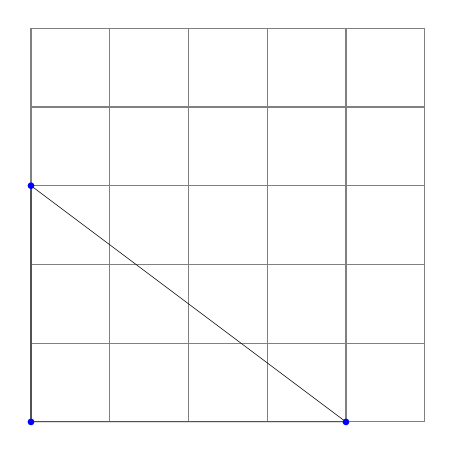
\begin{tikzpicture}
    % Init
    \tkzInit[xmax=5, ymax=5]
    \tkzGrid
    % 1. def point
    \tkzDefPoint(0, 0){A}
    \tkzDefPoint(4, 0){B}
    \tkzDefPoint(0, 3){C}
    % 2. def polygon
    \tkzDrawPolygon(A, B, C)
    % 3. show points before
    \tkzDrawPoints[color=blue](A, B, C)
\end{tikzpicture}
\end{bytes}
\columnbreak
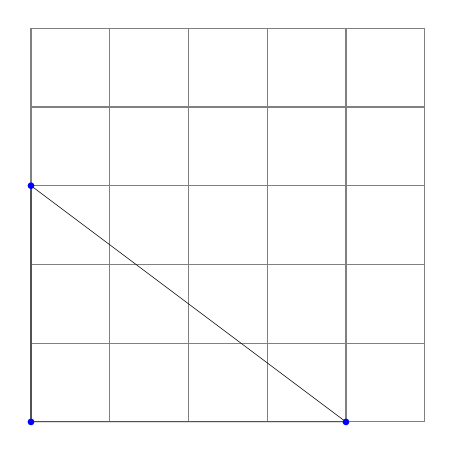
\begin{tikzpicture}
    % Init
    \tkzInit[xmax=5, ymax=5]
    \tkzGrid
    % 1. def point
    \tkzDefPoint(0, 0){A}
    \tkzDefPoint(4, 0){B}
    \tkzDefPoint(0, 3){C}
    % 2. def polygon
    \tkzDrawPolygon(A, B, C)
    % 3. show points before
    \tkzDrawPoints[color=blue](A, B, C)
\end{tikzpicture}  
\end{multicols}

\vspace*{4em}
\textbf{Warning}:
\begin{enumerate}[\lis 1)]
    \item \verb|\tkzDrawPoints[color=blue] (A, B, C)| is wrong \\
        Reason: $\longrightarrow$ \verb|space in [] and ()|.\\
        correct: $\longrightarrow$ \verb|\tkzDrawPoints[color=blue](A, B, C)|
    \item You don't need to load \verb|xfp, xcolor|
\end{enumerate}  


\clearpage
\subsection{Loop In Euclide}
\begin{multicols}{2}
    \begin{bytes}
\begin{tikzpicture}
    \foreach \an [count=\i] in {0,60,...,300}{
        \tkzDefPoint(\an:3){A_\i}
    }
    \tkzDrawPolygon(A_1,A_...,A_6)
    \tkzDrawPoints(A_1,A_...,A_6)
\end{tikzpicture}
    \end{bytes}
    \columnbreak
    \begin{tikzpicture}[scale=.7]
        \foreach \an [count=\i] in {0, 60, ..., 300}{
            \tkzDefPoint(\an:3){A_\i}
        }
        \tkzDrawPolygon(A_1, A_..., A_6)
        \tkzDrawPoints(A_1, A_..., A_6)
    \end{tikzpicture}
\end{multicols}

\textbf{Warning}: Becareful the Loop Method \verb|(A_1, A_..., A_6)|


\subsection{Reletive Point}
tikz 'scope' is one way of archieve reletive point define, while 
TiKZ-Euclide define a command

\lis\quad Original tikz method:
\begin{bytes}
\tkzDefPoint(2,3){A}
\begin{scope}[shift=(A)]
    \tkzDefPoint(90:5){B}
    \tkzDefPoint(30:5){C}
\end{scope}
\end{bytes}


\begin{center}
    \begin{tikzpicture}[scale=.7]
        \tkzSetUpLine[color=blue!60]
        \begin{scope}[rotate=0]
            \tkzDefPoint(2,3){A}
            \begin{scope}[shift=(A)]
                \tkzDefPoint(90:5){B}
                \tkzDefPoint(30:5){C}
            \end{scope}
        \end{scope}
        \tkzDrawPolygon(A,B,C)
        \tkzLabelPoints[above](B,C)
        \tkzLabelPoints[below](A)
        \tkzDrawPoints(A,B,C)
    \end{tikzpicture}
    \raise4em\hbox{\lrr{{\rm Rotate}~ 90^\circ}}
    \begin{tikzpicture}[scale=.7]
        \tkzSetUpLine[color=blue!60]
        \begin{scope}[rotate=90]
            \tkzDefPoint(2,3){A}
            \begin{scope}[shift=(A)]
                \tkzDefPoint(90:5){B}
                \tkzDefPoint(30:5){C}
            \end{scope}
        \end{scope}
        \tkzDrawPolygon(A,B,C)
        \tkzLabelPoints[above](B,C)
        \tkzLabelPoints[below](A)
        \tkzDrawPoints(A,B,C)
    \end{tikzpicture}
\end{center}

\lis\quad TiKZ-Euclide method:
\begin{bytes}
\tkzDefShiftPoint[A](30:3){B}
\end{bytes}


\begin{multicols}{2}
    \begin{bytes}
\begin{tikzpicture}
    \tkzDefPoint(0,0){A}
    \tkzDefShiftPoint[A](-4, 0){B}
    \tkzDefShiftPoint[A](120:4){C}
    \tkzDrawPolygon(A,B,C)
    \tkzDrawPoints(A,B,C)
    \tkzLabelPoints[below](A,B,C)
\end{tikzpicture} 
    \end{bytes}
    \begin{tikzpicture}
        \tkzDefPoint(0,0){A}
        \tkzDefShiftPoint[A](-4, 0){B}
        \tkzDefShiftPoint[A](120:4){C}
        \tkzDrawPolygon(A,B,C)
        \tkzDrawPoints(A,B,C)
        \tkzLabelPoints[right](A,B,C)
    \end{tikzpicture}
\end{multicols}


\clearpage
\let\point\tkzDefPoint
\subsection{Annotate}
Annotate an \texttt{angle} or {\ttfamily Asegment} is as simple as you had ever think:
\begin{bytes}
% 1. Draw coordinates
\tkzDrawXY[noticks,>=triangle 45]
% 2. Mark an Angle
\tkzMarkAngle[mark=none,->](I,O,P)
\tkzFillAngle[fill=blue!20, opacity=.5](I,O,P)
\tkzMarkRightAngle(I,O,P)
% 3. Annotate a segment, 'dim' is ioptional
\tkzDrawSegment[dim={$d$, <vertical distance>, above=<text vertical distance>}](O,P)
\end{bytes}

\begin{multicols}{2}
    \begin{bytes}
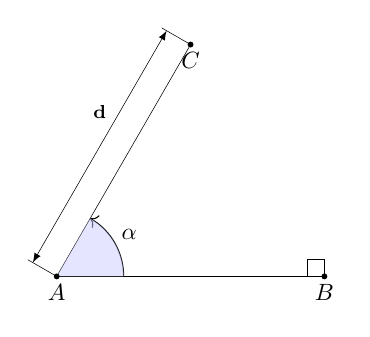
\begin{tikzpicture}[global scale=.85]
    \tkzDefPoint(0, 0){A}
    \tkzDefShiftPoint[A](4,0){B}
    \tkzDefShiftPoint[A](60:4){C}
    \tkzDrawSegment(A,B)
    \tkzDrawSegment[dim={$\mathbf{d}$, 1em, above=10pt}](A,C)
    \tkzMarkAngle[mark=none,->](B,A,C)
    \tkzFillAngle[fill=blue!20, opacity=.5](B,A,C)
    \tkzDefShiftPoint[B](90:3){D}
    \tkzMarkRightAngle(A,B,D)
    % Points Annotate
    \tkzLabelAngle[pos=1.25](B,A,C){$\alpha$}
    \tkzDrawPoints(A,B,C)
    \tkzLabelPoints[below](A,B,C)
\end{tikzpicture}
    \end{bytes}
\columnbreak
    % every node/.append style={scale=#1}
    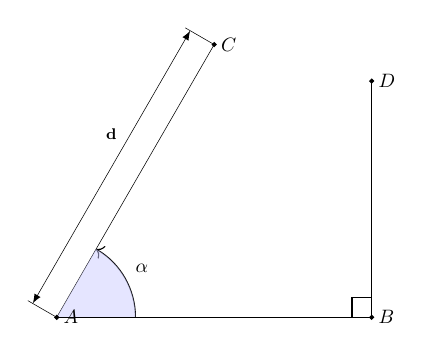
\begin{tikzpicture}[every node/.append style={scale=.7}]
        \tkzDefPoint(0, 0){A}
        \tkzDefShiftPoint[A](4,0){B}
        \tkzDefShiftPoint[A](60:4){C}
        \tkzDrawSegment[dim={$\mathbf{d}$, 1em, above=10pt}](A,C)
        \tkzMarkAngle[mark=none,->](B,A,C)
        \tkzFillAngle[fill=blue!20, opacity=.5](B,A,C)
        \tkzDefShiftPoint[B](90:3){D}
        \tkzMarkRightAngle(A,B,D)
        % show edge and points
        \tkzDrawSegment(A,B)
        \tkzDrawSegment(B,D)
        \tkzDrawPoints(A,...,D)
        % Points Annotate
        \tkzLabelAngle[pos=1.25](B,A,C){$\alpha$}
        \tkzLabelPoints[right](A,...,D)
    \end{tikzpicture}
\end{multicols}


\begin{multicols}{2}
    \begin{bytes}
% \usepackage{tkz-base} provide \tkzDrawXY
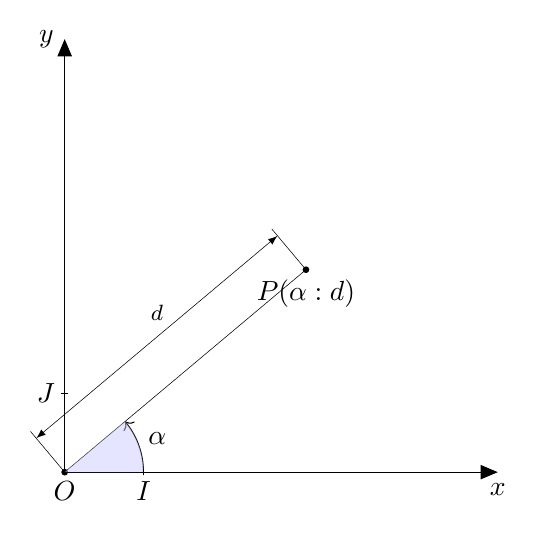
\begin{tikzpicture}[,scale=1]
    \tkzInit[xmax=5,ymax=5]
    \tkzDefPoints{0/0/O,1/0/I,0/1/J}
    \tkzDefPoint(40:4){P}
    \tkzDrawXY[noticks,>=triangle 45]
    \tkzDrawSegment[dim={$d$,16pt,above=6pt}](O,P)
    \tkzDrawPoints(O,P)
    \tkzMarkAngle[mark=none,->](I,O,P)
    \tkzFillAngle[fill=blue!20,opacity=.5](I,O,P)
    \tkzLabelAngle[pos=1.25](I,O,P){$\alpha$}
    \tkzLabelPoint(P){$P(\alpha : d )$}
    \tkzDrawPoints[shape=cross](I,J)
    \tkzLabelPoints(O,I)
    \tkzLabelPoints[left](J)
\end{tikzpicture}
    \end{bytes}
    \columnbreak
    \hspace*{3em}
    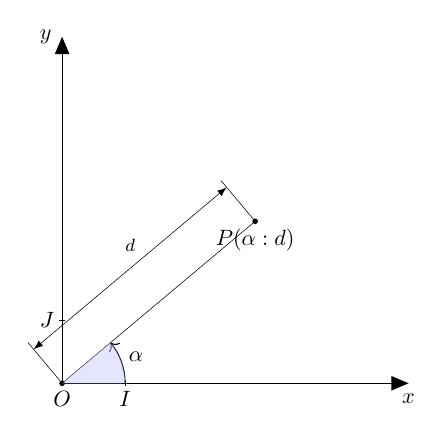
\begin{tikzpicture}[global scale=.8]
        \tkzInit[xmax=5,ymax=5]
        \tkzDefPoints{0/0/O,1/0/I,0/1/J}
        \tkzDefPoint(40:4){P}
        \tkzDrawXY[noticks,>=triangle 45]
        \tkzDrawSegment[dim={$d$,16pt,above=6pt}](O,P)
        \tkzDrawPoints(O,P)
        \tkzMarkAngle[mark=none,->](I,O,P)
        \tkzFillAngle[fill=blue!20,
        opacity=.5](I,O,P)
        \tkzLabelAngle[pos=1.25](I,O,P){$\alpha$}
        \tkzLabelPoint(P){$P
        (\alpha : d )$}
        \tkzDrawPoints[shape=cross](I,J)
        \tkzLabelPoints(O,I)
        \tkzLabelPoints[left](J)
    \end{tikzpicture}
\end{multicols}


\clearpage
\section{Get Ponits}
Use predifined Command, We can make get some tipycial points, such as 
\texttt{midpoint, center, circumcenter, orthocenter, incenter},
in a Euclide graph, Such as \texttt{segment, triangle, square, circle}. 

To get the target point, we need to use:
\begin{bytes}
\tkzGetPoints{<target point alias>}
\end{bytes}

just after the cmd, such as \verb|\tkzDefMidPoint(A,B)|. There is an Example:
\begin{multicols}{2}
    \begin{bytes}
\begin{tikzpicture}[scale=1]
    \tkzDefPoint(2,3){A}
    \tkzDefPoint(4,0){B}
    \tkzDefMidPoint(A,B) \tkzGetPoint{C}
    \tkzDrawSegment(A,B)
    \tkzDrawPoints(A,B,C)
    \tkzLabelPoints[right](A,B,C)
\end{tikzpicture}        
    \end{bytes}
    \begin{tikzpicture}[scale=1]
        \tkzDefPoint(2,3){A}
        \tkzDefPoint(4,0){B}
        \tkzDefMidPoint(A,B) \tkzGetPoint{C}
        \tkzDrawSegment(A,B)
        \tkzDrawPoints(A,B,C)
        \tkzLabelPoints[right](A,B,C)
    \end{tikzpicture}
\end{multicols}

Just make it a command, and you can get the point using one command:
\begin{bytes}
% \getmidpoint[<your target point alias>]{pt1, pt2}
\newcommand{\getmidpoint}[2][]{%
    \tkzDefMidPoint(#2) \tkzGetPoint{#1}
}
\end{bytes}
\newcommand{\getmidpoint}[2][]{%
    \tkzDefMidPoint(#2) \tkzGetPoint{#1}
}

\begin{multicols}{2}
    \begin{bytes}
\begin{tikzpicture}[scale=1]
    \tkzDefPoint(2,3){A}
    \tkzDefPoint(4,0){B}
    \getmidpoint[C]{A,B}
    \tkzDrawSegment(A,B)
    \tkzDrawPoints(A,B,C)
    \tkzLabelPoints[right](A,B,C)
\end{tikzpicture}
    \end{bytes}
    \begin{tikzpicture}[scale=1]
        \tkzDefPoint(2,3){A}
        \tkzDefPoint(4,0){B}
        \getmidpoint[C]{A,B}
        \tkzDrawSegment(A,B)
        \tkzDrawPoints(A,B,C)
        \tkzLabelPoints[right](A,B,C)
    \end{tikzpicture}
\end{multicols}



Or you can use More Advanced commnad in \LaTeX{}3 to archieve the goal:
\begin{bytes}
\tl_const:Nn \c_partcmd_i
% #1 = ii, iii, etc
% combine the str, then translate it to a Macro
\tl_use:c {c_partcmd_#1}
\end{bytes}





\end{document}